\chapter{Risultati ottenuti}

Sono state eseguite numerose prove che hanno \textit{confutato} quanto detto fino ad ora riguardo i vantaggi e problemi della parallelizzazione.\newline

\noindent In caso di immagine di \textit{dimensione troppo piccola}, i guadagni di performance vengono meno a causa dell'\textit{overhead} di creazione e comunicazione dei processi. L'esecuzione sequenziale ha sempre la meglio.

\begin{figure}[H]
	\centering
	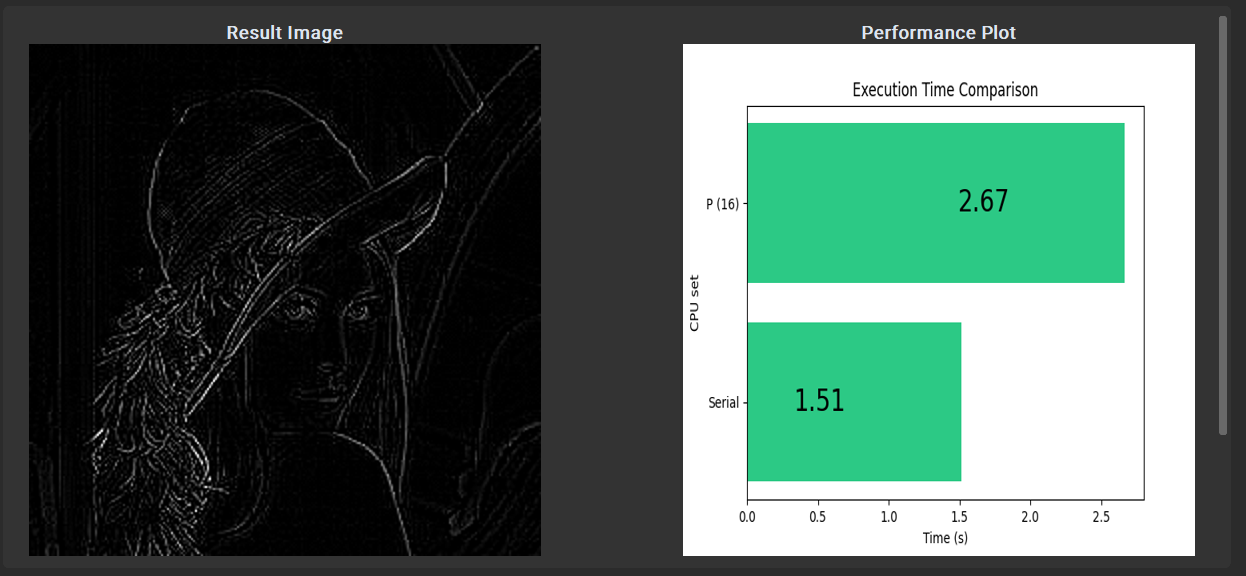
\includegraphics[width=\linewidth]{too-small}
	\caption{Esempio di parallelizzazione Lenna 256x256}
\end{figure}

\noindent In caso di immagine di \textit{dimensioni medie}, si hanno guadagni di performance con suddivisioni di piccolo taglio, tali guadagni vengono prima attenutati e successivamente persi man mano che aumentano le suddivisioni, sempre a causa dell'\textit{overhead} di creazione e comunicazione dei processi.

\begin{figure}[H]
	\centering
	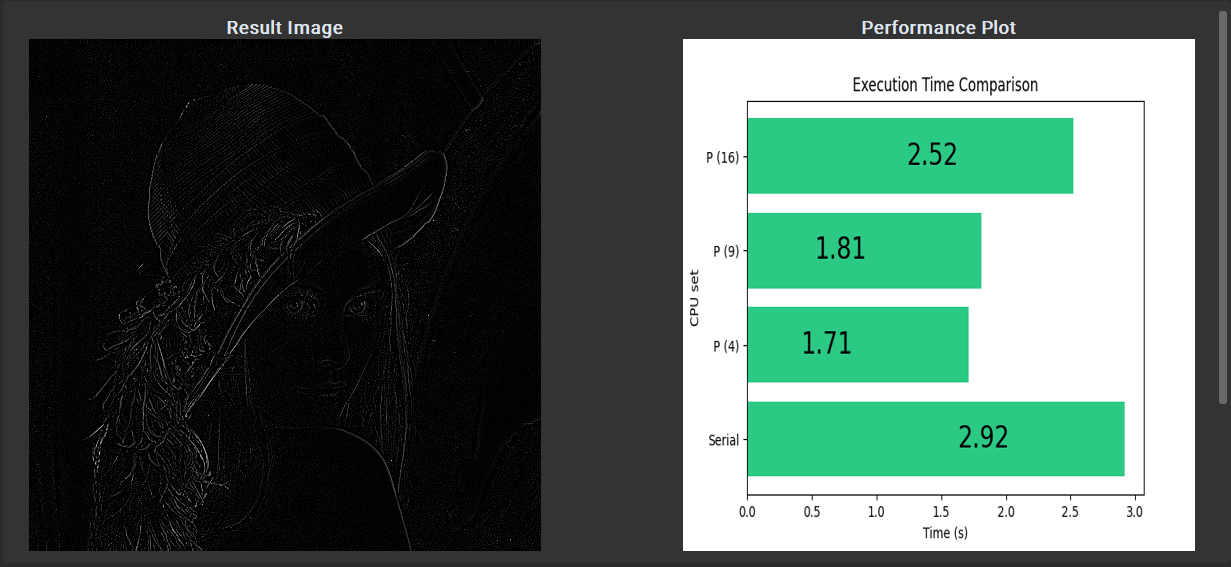
\includegraphics[width=\linewidth]{medium}
	\caption{Esempio di parallelizzazione Lenna 512x512}
\end{figure}


\noindent In caso di immagine di \textit{dimensioni grandi}, si hanno guadagni di performance evidenti. L'\textit{overhead} di creazione e comunicazione dei processi diventa meno trascurabile all'aumentare delle suddivisioni.

\begin{figure}[H]
	\centering
	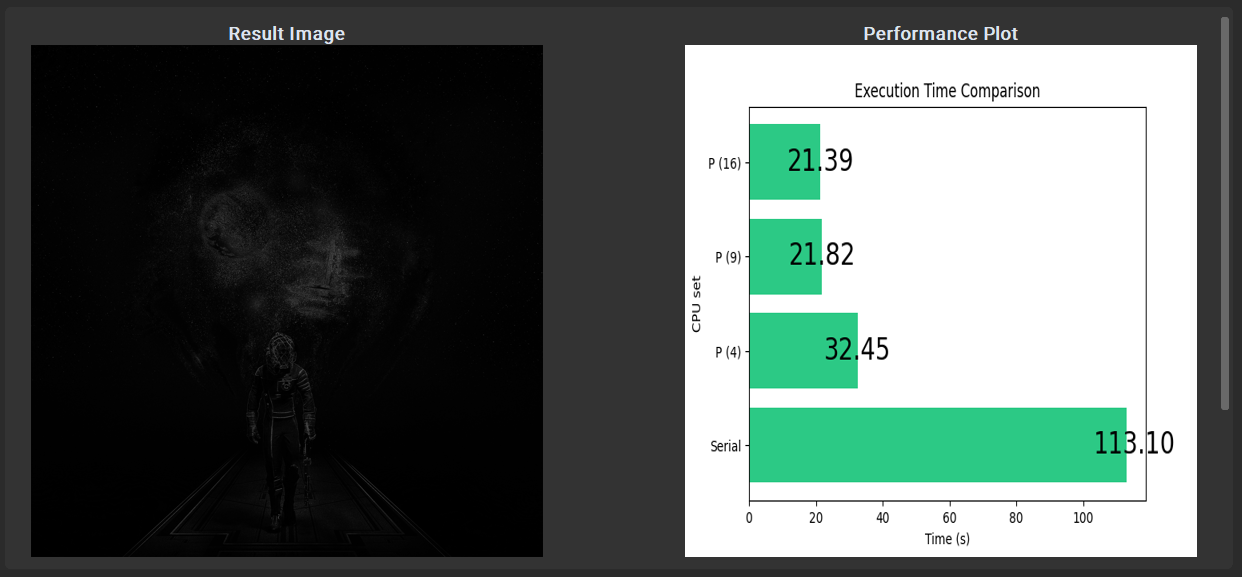
\includegraphics[width=\linewidth]{large}
	\caption{Esempio di parallelizzazione Prey 4000x4000}
\end{figure}


\noindent Infine, si è tentato un confronto fra la convoluzione implementata a mano e quella offerta dalla libreria \textit{SciPy}, il risultato è alquanto prevedibile in quanto tale libreria fa uso di implementazioni in C.
In tale configurazione il collo di bottiglia è rappresentato dalla tecnica di parallelizzazione di Python che degrada le performance offerte dal C.
\begin{figure}[H]
	\centering
	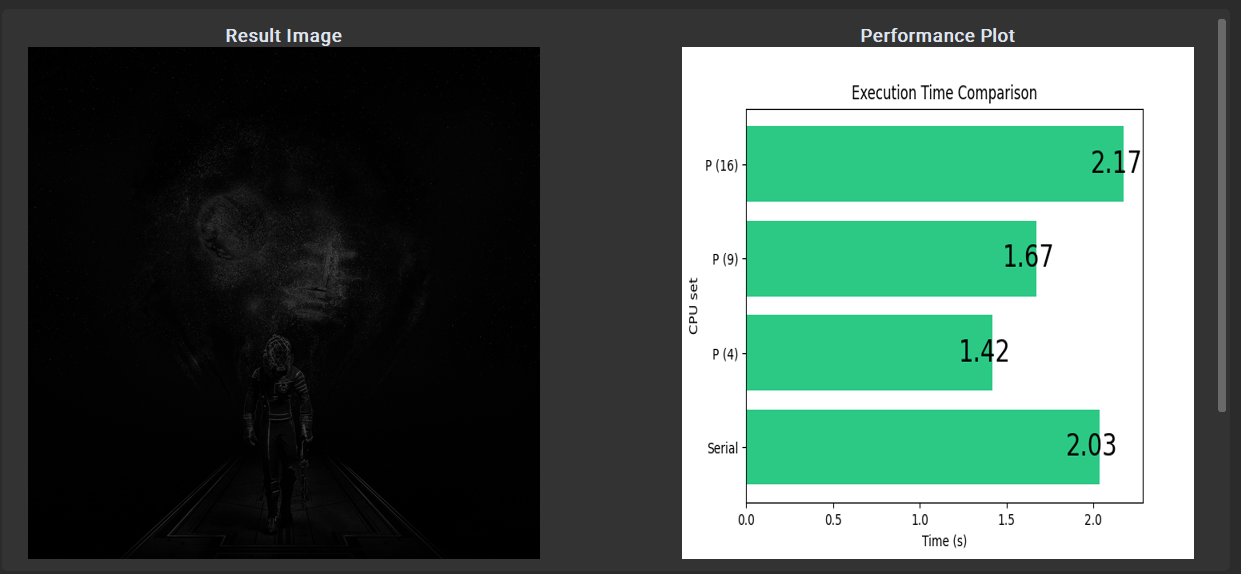
\includegraphics[width=\linewidth]{lib-conv}
	\caption{Esempio di parallelizzazione SciPy Prey 4000x4000}
\end{figure}